% Section IV: GaitNet on OCS2, from the benchmark the author sent on
% 2026-10-14 (OCS2-fitted IDM, depth-camera terrain, 0-70 % voids,
% 0.05-0.25 m/s, 10 trials per cell). Plots: figures/ocs2_results.pdf, made
% by figures/plot_ocs2_results.py, which holds the per-cell data. Pooled
% values: \corlOcs* macros in constants.tex.

\section{Simulation Experiments}
\label{sec:experiments}

We ask three questions. (Q1)~Does the frozen GaitNet succeed on OCS2 as
often as OCS2's own trot as voids get denser and commands faster?
(Q2)~Does GaitNet need to swing more than one leg at a time?
(Q3)~Do the IDM and the candidate mixer matter?

\subsection{Setup}
\label{subsec:exp-setup}

We deploy iteration \corlTrainingIterations{} of one training run, frozen
after training \verify{(to be confirmed for the OCS2 benchmark)}. The
run's settings changed while it trained. It used omnidirectional
commands for its first \corlOmniIterations{} iterations, then forward
commands without the IDM until iteration \corlIdmStartIteration, and
with the IDM in the loop after that. It was not seeded and used
$\corlTotalTransitions$ transitions, about \corlTrainHours\,h on one
NVIDIA RTX PRO 6000.

We run GaitNet on OCS2 in Gazebo (Sec.~\ref{subsec:method-deployment}),
with terrain from the simulated depth camera and the IDM fitted on
OCS2's own steps (Sec.~\ref{subsec:method-idm}). Each world is a strip
of pillars in which each tile is a real drop with probability equal to
the void fraction. We test eight void fractions, from 0 to
\corlOcsMaxVoidPct\%, and five forward speeds, from \corlOcsSpeedMin{}
to \corlOcsSpeedMax\,m/s, with \corlOcsTrialsPerCell{} trials for each
pair, and 14 for OCS2's own trot in the comparison by speed. The fastest command lies above the \corlCmdVxMax\,m/s that
GaitNet was trained on. A trial succeeds if the robot does not fall and
walks at least half the commanded distance \verify{(trial length to be
stated)}; leaving the strip also counts as a failure.
\pending{The benchmark's world seeds will be listed.}

We compare five conditions. All except OCS2's own trot keep OCS2's NMPC
and WBC but replace its gait scheduler and foothold choice with the
planner's steps, so the comparison focuses on the planner rather than
the tracker.
\begin{enumerate}
  \item GaitNet: as deployed; up to two legs may swing at once.
  \item OCS2's own trot: OCS2's perceptive trot, with its own gait
    scheduler and footholds \verify{(on the same camera)}.
  \item GaitNet-Single: only one leg may swing at a time.
  \item GaitNet, no IDM: the chosen landing point is sent to OCS2
    unchanged.
  \item Per-candidate + IDM: the per-candidate network of
    \cite{Sullivan2025} (Sec.~\ref{subsec:method-network}), which scores
    each candidate on its own, with the same IDM \verify{(checkpoint to
    be stated)}.
\end{enumerate}
\verify{GaitNet-Single and GaitNet, no IDM use GaitNet's weights.}

\begin{figure*}[t]
  \centering
  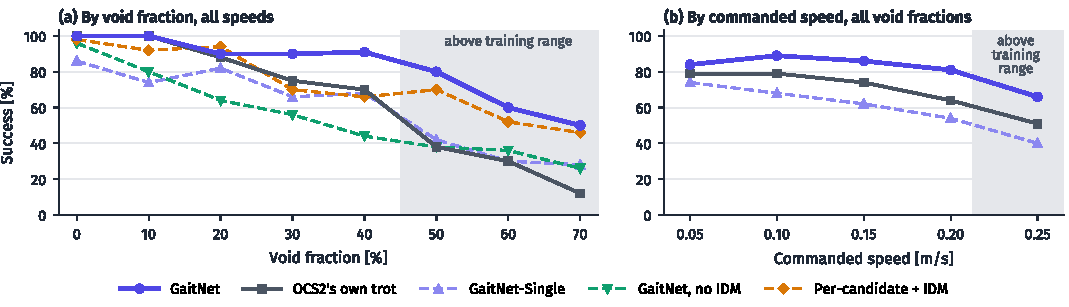
\includegraphics[width=\textwidth]{figures/ocs2_results}
  \caption{Success on OCS2 with depth-camera terrain. (a)~By void
    fraction, pooled over the five commanded speeds (50 trials per
    point). (b)~By commanded speed, pooled over the eight void fractions
    (80 trials per point, 112 for OCS2's own trot); GaitNet was trained up to
    \corlCmdVxMax\,m/s.}
  \label{fig:ocs2-results}
\end{figure*}

\subsection{Comparison with OCS2's Own Trot}
\label{subsec:exp-transfer}

GaitNet matches OCS2's own trot on sparse voids and does better as the
voids get denser (Fig.~\ref{fig:ocs2-results}a). Both succeed in every
trial up to 10\% voids and are within two points at 20\%. From 30\% voids on,
GaitNet leads at every void fraction, with \corlOcsDenseFull\% against
\corlOcsDenseTrot\% success over 40--\corlOcsMaxVoidPct\% voids.
At \corlOcsMaxVoidPct\% voids, GaitNet still succeeds in half of the trials and OCS2's own trot in few. GaitNet also leads at every
commanded speed (Fig.~\ref{fig:ocs2-results}b) and walks closer to
the commanded speed, at about 92\% of it against about 84\% for
OCS2's own trot \verify{(mean over trials)}. Both lose success at
\corlOcsSpeedMax\,m/s, above GaitNet's training range.

\subsection{Ablations}
\label{subsec:exp-why}

Overlapping swings matter (Q2). Under a one-swing limit, GaitNet still
walks, but it succeeds less often at every void fraction and every
speed, \corlOcsAllSingle\% against \corlOcsAllFull\% on average over
void fractions, and the gap is largest on dense voids and at the
faster commands. Because GaitNet was never trained under this limit,
this shows that GaitNet relies on occasionally swinging two legs
together, not that overlap is better in general.

The IDM matters most (Q3). Without it, GaitNet's success falls from
\corlOcsAllFull\% to \corlOcsAllNoIdm\% on average over void fractions.
Only on ground without voids, where a missed landing costs little,
does GaitNet do well without it.

Comparing candidates matters on dense voids. The per-candidate network,
which has neither the candidate mixer nor the history, with the same IDM, is about as good as GaitNet up to 20\% voids but
falls behind from 30\% on, with \corlOcsDenseMlp\% against
\corlOcsDenseFull\% over 40--\corlOcsMaxVoidPct\% voids. \verify{The two
networks also differ in training history}, so this is not a fully
controlled comparison.
